\documentclass{article}
\usepackage[spanish]{babel}
\usepackage[utf8]{inputenc}
\usepackage{amsmath,amssymb,amsthm}
\usepackage{graphicx}
\usepackage{fancyhdr}
\usepackage{geometry}

%Información del documento:
\newcommand{\departamento}{Magister en Ciencia de Datos}
\newcommand{\titulo}{Laboratorio 1}
\newcommand{\curso}{MDS7203 Modelos Generativos Profundos}
\newcommand{\autor}{Fernando Fêtis Riquelme}
\newcommand{\fecha}{\today}
\newcommand{\prob}{\mathbb{P}}
\newcommand{\normal}{\mathcal{N}}

%Configuración de página:
\geometry{letterpaper,margin=2.5cm,tmargin=3.5cm}
\fancyhead[L]{\curso}
\fancyhead[R]{\titulo}
\pagestyle{fancy}

\begin{document}

%Portada:
\begin{titlepage}
	\centering
	
\includegraphics[width=0.5\textwidth]{imgs/uchile}\\
	\begin{Large}
		\begin{scshape}
			Facultad de Ciencias Físicas y Matemáticas\\
			\departamento\\
			\vspace{2.5cm}\Huge\titulo\\
		\end{scshape}
		\vspace{0.5cm}\curso\\
		\vspace{4cm}\autor
	\end{Large}
	\vfill\fecha
\end{titlepage}

\tableofcontents\thispagestyle{empty}
\newpage\setcounter{page}{1}

% Pregunta 1.
\section{Sampling usando Metropolis-Hastings}

\subsection{Distribución half-normal}

Se generó una muestra a partir de la distribución $\mu\sim\text{HalfNormal}(10)$. Con esto, se fijó $\mu\approx2.72$.

\subsection{Generación de muestras gaussianas}

Se generaron $n=42$ muestras $\{x_i\}_{i=1}^n$ independientes a partir de la distribución $x\sim\mathcal{N}(\mu,5)$. En la Figura 1 (izquierda) se puede ver un histograma de las muestras.

\begin{figure}[h]
	\centering
	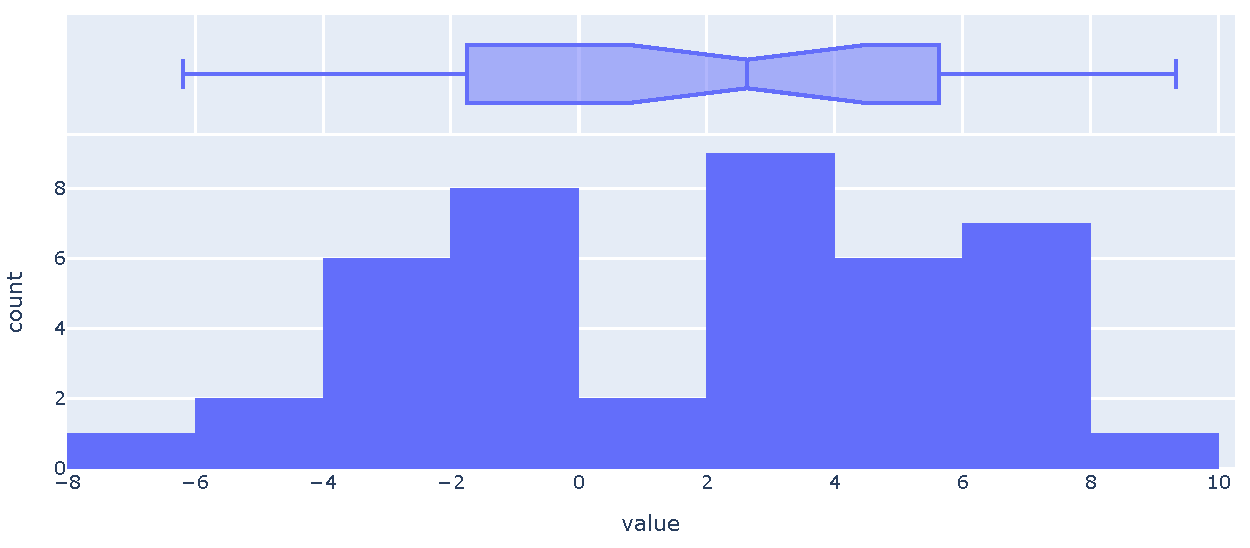
\includegraphics[width=0.45\textwidth]{imgs/p1.2.pdf}
	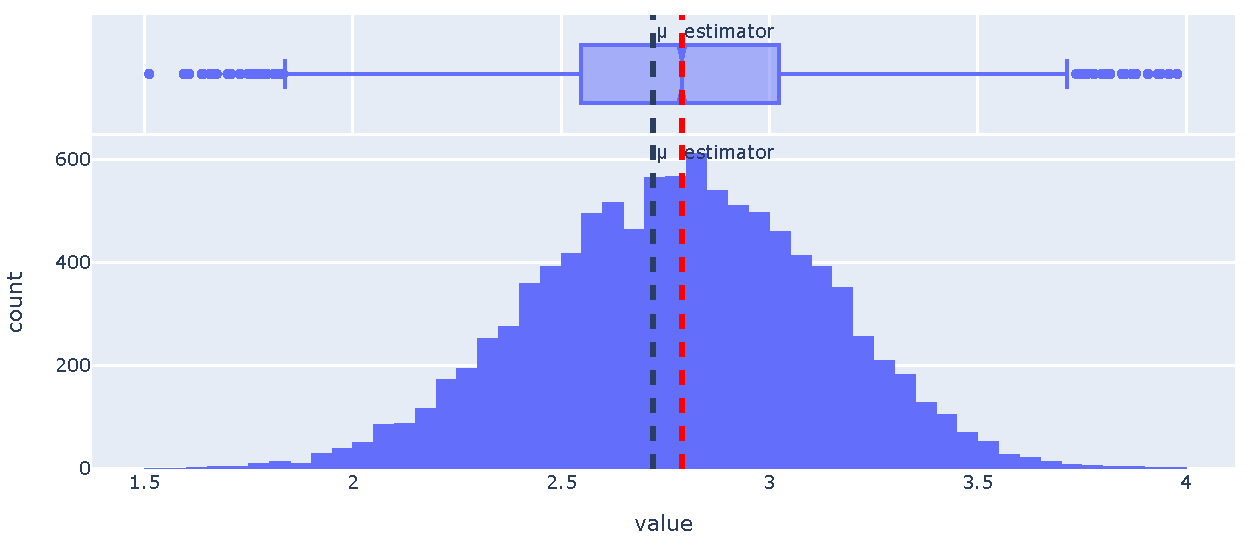
\includegraphics[width=0.45\textwidth]{imgs/p1.4.pdf}
	\caption{(izquierda) histograma de $\{x_i\}_{i=1}^n$. (derecha) histograma de $\{\hat{\mu}_i\}_{i=1}^m$ junto a su mediana y el valor real de $\mu$.}
	
\end{figure}

\subsection{Distribución posterior para $\mu$}

Primero se determinará la densidad de $\mu\sim\text{HalfNormal}(\sigma^2)$, ie, $\mu=|X|$, donde $X\sim\mathcal{N}(0,\sigma^2)$. Para esto, sea $f(x)=|x|$, entonces $f'(x)=\text{sgn}(x)$ c.t.p. y $f^{-1}(\mu)=\{\pm\mu\}$. Luego, para $\mu>0$:

\begin{equation*}
	p_\mu(\mu) = \sum_{x\in f^{-1}(\mu)} |f'(x)|^{-1} p_x(x) = f_x(\mu) + f_x(-\mu)=\sqrt{\frac{2}{\pi\sigma^2}} \exp\left(\frac{-\mu^2}{2\sigma^2}\right)
\end{equation*}

Luego, para la distribución posterior, considerando que los $x_i|\mu\sim\mathcal{N}(\mu,s^2)$ son independientes:
\begin{align*}
	p(\mu|x_1,\ldots,x_n) &\propto p_{x|\mu}(x_1,\ldots,x_n|\mu) p_\mu(\mu) = \left(\prod_{k=1}^n p(x_k|\mu)\right)p_\mu(\mu)\\
	&\propto \left(\prod_{k=1}^n \exp\left(\frac{-1}{2s^2}(x_k-\mu)^2\right)\right) \exp\left(\frac{-\mu^2}{2\sigma^2}\right)=\exp\left(\frac{-\mu^2}{2\sigma^2} - \frac{1}{2s^2} \sum_{k=1}^n (x_k-\mu)^2 \right)
\end{align*}

Esta es la distribución desde la que se buscará generar muestras utilizando Metropolis-Hastings.

\subsection{Sampling usando Metropolis-Hastings}

En esta parte se generaron $m=10000$ muestras $\hat{\mu} \sim p(\cdot|x_1,\ldots,x_n)$ utilizando Metropolis-Hastings. Para esto, se generaron nuevos candidatos a estados de la cadena de Markov usando una distribución gaussiana centrada en el estado actual: $x_{t+1}|x_t \sim \mathcal{N}(x_t, 1)$. Se decidió utilizar esta distribución ya que su soporte es todo $\mathbb{R}$ y además es simétrica (vista como kernel), lo cual garantiza que que la matriz de transición asociada a la cadena de Markov y la medida de probabilidad $p(\cdot|x_1,\ldots,x_n)$ están en balance detallado, lo cual a su vez garantiza que la distribución deseada es efectivamente la medida invariante de la cadena de Markov.

Por otra parte, se omitieron las primeras 5000 muestras de la CM (burn in) para esperar a que la cadena se estabilice a su distribución invariante. Además, se eligieron muestras cada 10 estados consecutivos de la CM (thinning) con el fin de disminuir la autocorrelación entre las muestras consecutivas.

Tomando como estimador de $\mu$ a la mediana empírica de $\{\mu_i\}_{i=1}^m$, se obtuvo un estimador $\hat{\mu}\approx 2.789$, obteniendo un error relativo del $2.6\%$. Las muestras y la mediana pueden verse en la Figura 1 (derecha).

\subsection{Comparación con valor real para distinta cantidad de evidencia}

Se realizó el experimento anterior para $n\in\{20, 40, 60, 80, 100\}$. Todos los otros parámetros quedaron iguales. En la Figura 2 se observa la distribución empírica que se obtuvo para los distintos valores de $n$. Se espera que al aumentar $n$, la distribución posterior desde la que se generan los puntos esté más concentrada en $\mu$ (ya que se tiene más información para estimar su valor). Sin embargo, aquí se observa que no hay un patrón claro entre $n$ y la cercanía a $\mu$. Esto puede deberse a la inestabilidad numérica que ocurre al trabajar con un sampler gaussiano ya que se está trabajando con la verosimilitud y no con la log-verosimilitud como se hace generalmente. Esto se confirma al trabajar con $n>500$, donde la distribución cada vez se aleja más. 

\begin{figure}[h]
	\centering
	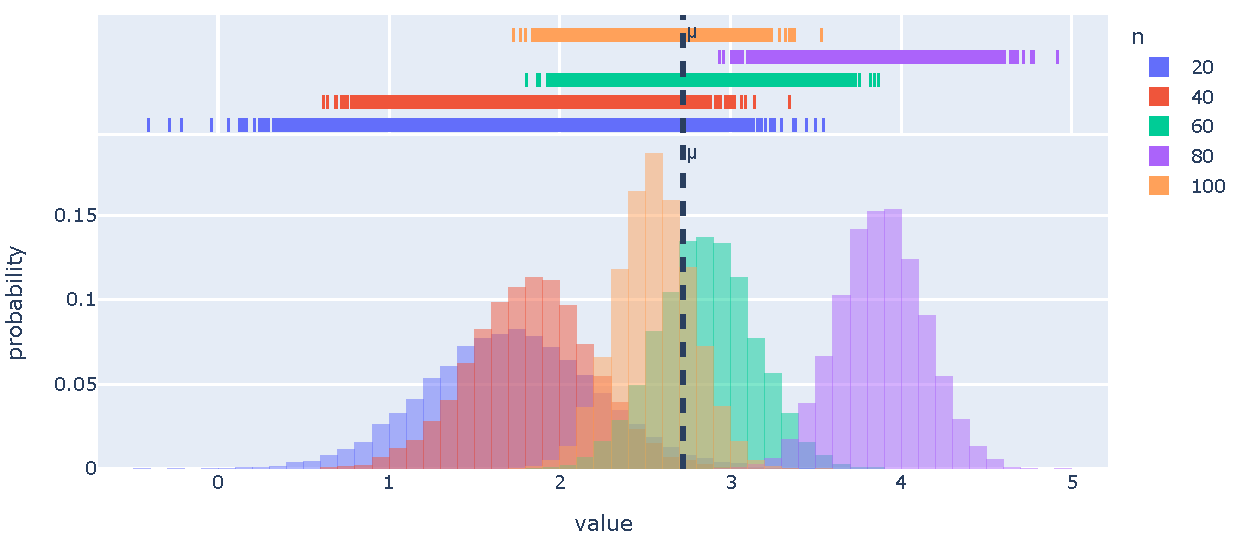
\includegraphics[width=1\textwidth]{imgs/p1.5.pdf}
	\caption{Histograma de $\{\hat{\mu}_i\}_{i=1}^m$ para distintos valores de $n$, junto al valor real de $\mu$.}
	
\end{figure}

\subsection{Experimento para una mezcla de gaussianas}

Para $\mu,\lambda\in\mathbb{R}^3$ se propusieron las distribuciones $\mu\sim \text{NMV}((-1, 0, 1), I_3)$ y $\lambda\sim\text{Cat}(0.3, 0.5, 0.2)$. Con esto, se propuso el GMM $x\sim \sum_{i=1}^3 \lambda_i \mathcal{N}(\mu_i, 1)$. De esta forma, se fijó la muestra generada $\mu=(-1.4, -0.6, 0.01)^\top$ y se generaron $n$ muestras $\{x_i\}_{i=1}^n$ del GMM.

Para inferencia (unidimensional), se calculó la posterior $\mu_1|x_1,\ldots,x_n,\mu_2,\mu_3, \lambda$ (ie, considerando conocidos los otros parámetros). Luego, se generaron $m$ muestras a partir de esta distribución utilizando Metropolis-Hastings. Como estimador de $\mu_1$ se consideró nuevamente a la mediana. Los resultados para distintos valores de $n$ se pueden ver en la Figura 3.

Observamos que se obtiene un error relativo más alto que en el caso anterior. Esto se debe a que los datos usados para hacer inferencia provienen de una distribución multimodal. Acercando los centroides de la GMM o dándole una mayor probabilidad categórica ($\lambda_1$) a la primera gaussiana el error relativo debería disminuir, ya que es precisamente esta la distribución que importa para hacer inferencia sobre el parámetro $\mu_1$.

\begin{figure}[h]
	\centering
	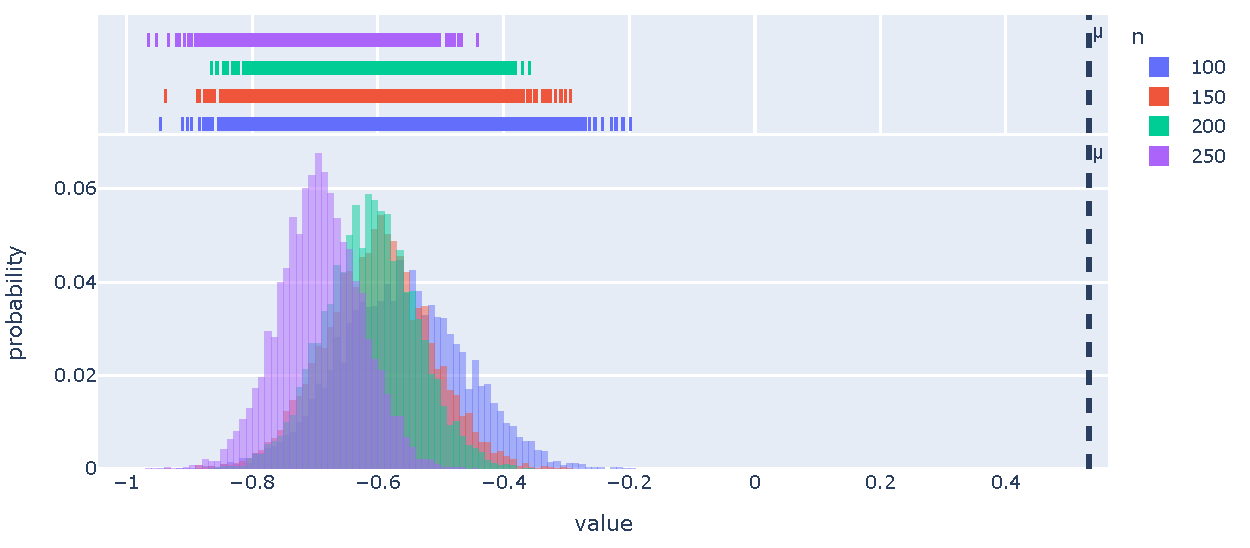
\includegraphics[width=1\textwidth]{imgs/p1.6.pdf}
	\caption{Histograma de $\{\hat{\mu_1}_i\}_{i=1}^m$ para distintos valores de $n$, junto al valor real de $\mu_1$.}
	
\end{figure}


% Pregunta 2.
\section{Modelo gráfico para la rinitis alérgica}

\subsection{Formulación como una red bayesiana}

Se considerará el siguiente modelo gráfico, donde la ausencia de aristas entre dos nodos indica independencia condicional:

\begin{figure}[h]
	\centering
	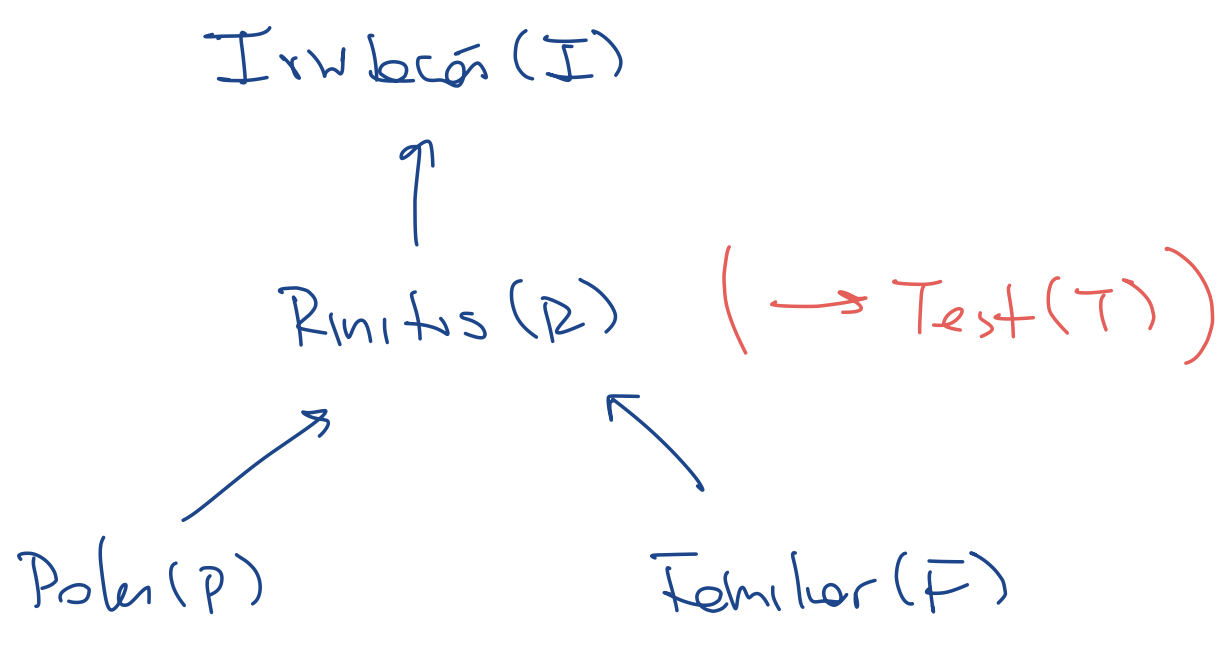
\includegraphics[width=0.6\textwidth]{imgs/p2.1.png}
	\caption{DAG asociado al modelo gráfico propuesto.}
\end{figure}

Donde se está considerando que cada variable (condicional) distribuye Bernoulli, por lo que depende de un único parámetro. Por otra parte, gracias a la regla de la cadena y la independencia condicional:

\begin{equation*}
	\prob(P,F,R,I) = \prob(P)\prob(F)\prob(R|P,F)\prob(I|R)
\end{equation*}

\newpage
\subsection{Probabilidad condicional de tener rinitis}

Por regla de Bayes, $\prob(R|I) = \frac{\prob(I|R)\prob(R)}{\prob(I)}$. Con probabilidades totales se obtienen las marginales faltantes:

\begin{align*}
	\prob(R) &= \sum_{P,F} \prob(R|P,F)\prob(P,F) = \sum_{P,F} \prob(R|P,F)\prob(P)\prob(F)\\
	\prob(I) &= \sum_{R} \prob(I|R)\prob(R)
\end{align*}

Por lo tanto:

\begin{equation*}
	\prob(R|I) = \frac{\prob(I|R)\sum_{P,F} \prob(R|P,F)\prob(P)\prob(F)}{\sum_{R'} \prob(I|R') \sum_{P,F} \prob(R'|P,F)\prob(P)\prob(F)}
\end{equation*}

\subsection{Incorporación de test alérgico en el modelo}

Si bien es posible integrar la nueva variable de varias formas, para este caso se considerará que $T|R$ es independiente de las otras variables del modelo (es decir, el resultado del test dependerá unicamente de la variable latente asociada a tener rinitis). Para este caso, se tienen dos distribuciones condicionales para $R$: 

\begin{itemize}
	\item Si solo se considera el resultado del test:
	\begin{equation*}
		\prob(R|T) = \frac{\prob(T|R)\prob(R)}{\prob(T)} = \frac{\prob(T|R)\prob(R)}{\sum_{R'} \prob(T|R')\prob(R')}
	\end{equation*}

	\item Si también se considera la irritación en nariz y ojos:
	\begin{equation*}
		\prob(R|T,I) = \frac{\prob(T,I|R)\prob(R)}{\prob(T,I)} = \frac{\prob(T,I|R)\prob(R)}{\sum_{R'} \prob(T,I|R')\prob(R')} = \frac{\prob(T|R)\prob(I|R)\prob(R)}{\sum_{R'}\prob(T|R')\prob(I|R')\prob(R')}
	\end{equation*}
\end{itemize}

\subsection{Polen como una distribución continua}

Hasta el momento se ha tratado el polen como una variable discreta, indicando si hay o no polen en el ambiente, aunque también es posible tratarlo como una variable continua que represente la cantidad de polen en el ambiente. Suponiendo que $Y_{\text{polen}} = \text{HalfNormal}{(\sigma^2)}$, se observa lo siguiente en

\begin{itemize}
	\item $\text{Mode}(Y_{\text{polen}})=0$, por lo que la ausencia de polen es el estado de mayor densidad, la cual empieza a disminuir a medida que aumenta el polen en el ambiente. Esto puede verse en la Figura 5.
	
	\begin{figure}[h]
		\centering
		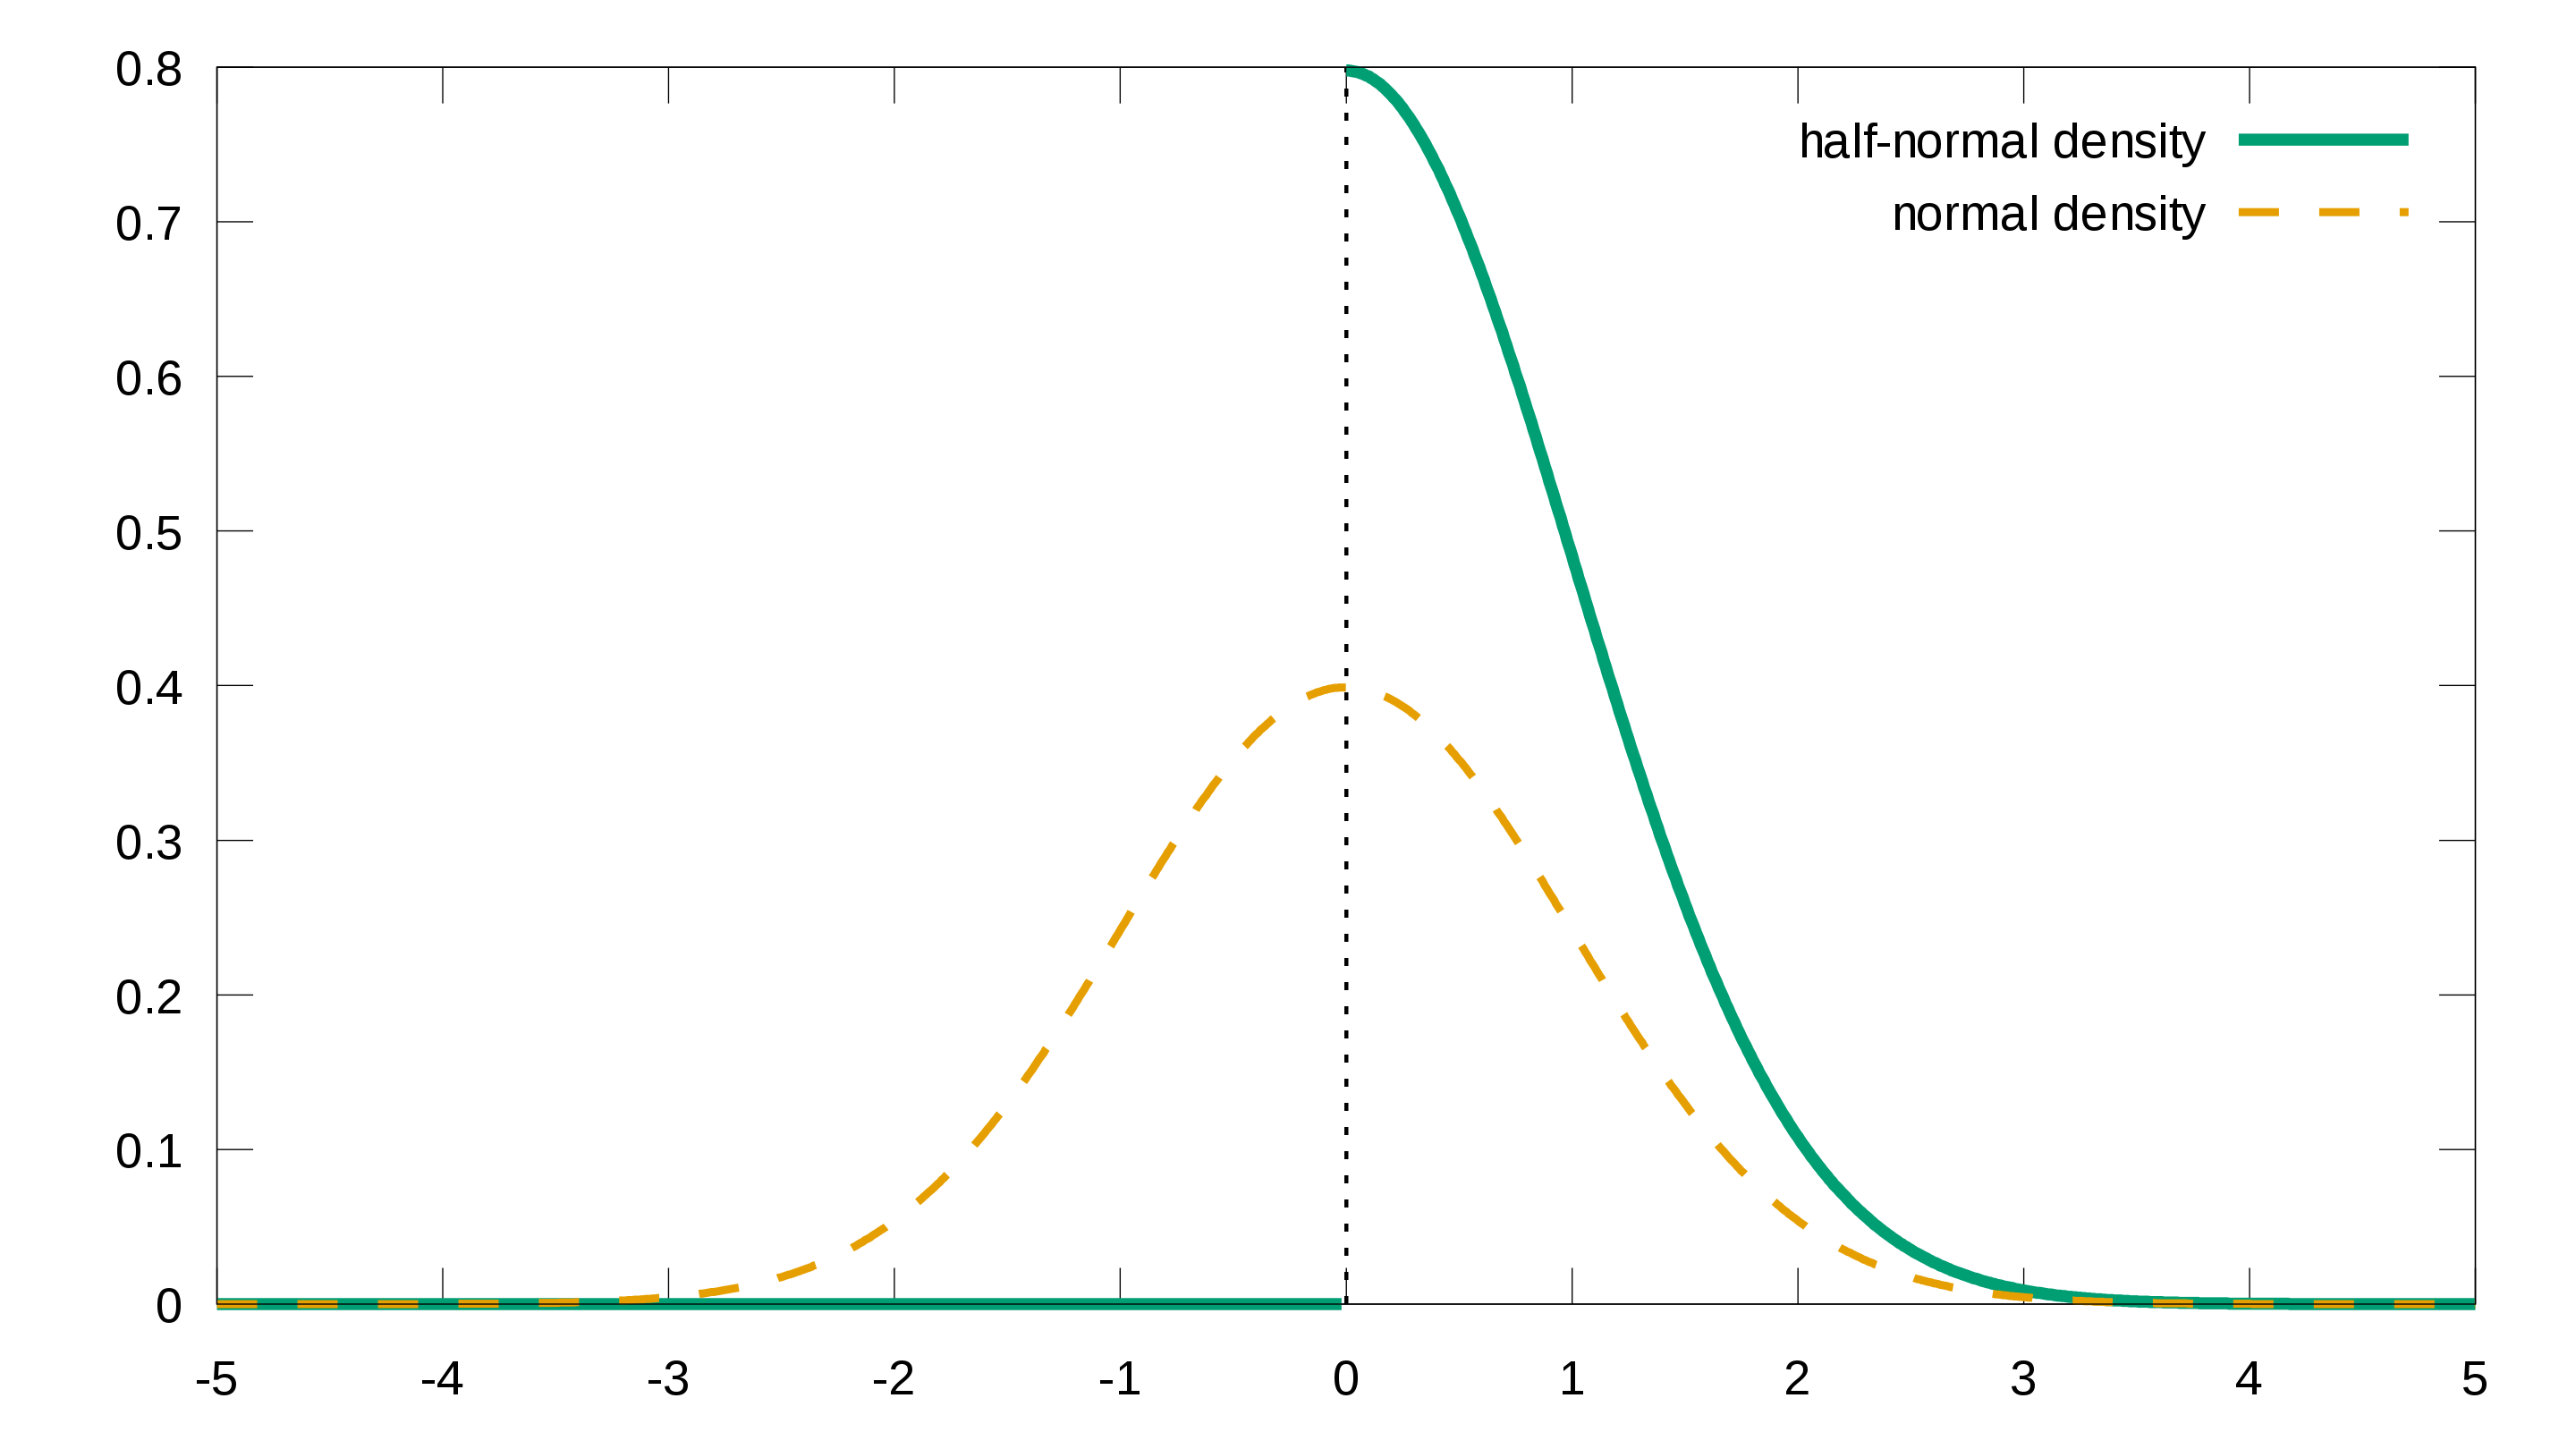
\includegraphics[width=0.5\textwidth]{imgs/p2.6.png}
		\caption{Densidad para $Y_{\text{polen}} = \text{HalfNormal}{(1)}$. Imagen obtenida de Wikipedia.}
	\end{figure}

	\item $\mathbb{E}(Y_{\text{polen}})=\sigma\sqrt{\frac{2}{\pi}}$ y $\text{Var}(Y_{\text{polen}})=\sigma^2 \left(1-\frac{2}{\pi}\right)$, por lo que para aumentar la cantidad de polen esperada es necesario aumentar la varianza en el modelo.
	\item Por lo anterior, puede ser mejor utilizar otra distribución para representar la cantidad de polen, como por ejemplo la distribución gamma (tiene soporte positivo y se pueden controlar más libremente sus momentos).
\end{itemize}

Comparando este modelo con el modelo anterior, se destaca que:

\begin{itemize}
	\item Este modelo puede ser más representativo de la realidad ya que por lo general la cantidad presente de una sustancia es más informativo que la presencia o no de dicha sustancia (en este caso, el polen).
	\item La distribución ahora es continua, por lo que en las fórmulas anteriores se debe cambiar probabilidad (masa) por densidad y se debe integrar en vez de sumar al usar probabilidades totales condicionando sobre la cantidad de polen.
	\item En el modelo discreto, la presencia de polen se modela como una distribución Bernoulli($p$), lo que permite fijar $p\sim0$ para indicar que es muy poco probable la presencia de polen. En el modelo continuo, el evento que representa la ausencia de polen tiene probabilidad nula (HalfNormal es una distribución no atómica).
\end{itemize}

\subsection{Predicción del polen usando un HMM}

Para este parte, se tratará la cantidad de polen, $P$ (distribución continua), como una variable oculta y la irritación en nariz y ojos, $I$ (distribución binaria), como variable observable.

Para inducir que el pasado y el futuro sean independientes dado el estado actual (todo esto para $P$), el problema será modelado como un HMM $P\to I$ ya que la condición anterior es una caracterízación de una cadena de Markov.

Por lo tanto, dadas las observaciones $(I_t)_{t=1}^n$ (cada 30 minutos) indicando la presencia de irritación en nariz y ojos, estas tienen asociados estados ocultos $(P_t)_{t=1}^n$ que indican la cantidad de polen en el ambiente. De esta forma, el modelo propuesto es el siguiente:
\begin{equation*}
	p(I,P) = p(P_1)p(I_1|p_1) \prod_{t=2}^n p(I_t|P_t)p(P_t|P_{t-1})
\end{equation*}

Donde $I:=(I_t)_{t=1}^n$ y $P:=(P_t)_{t=1}^n$ son las dos series de tiempo del problema. Luego, para obtener la densidad asociada a la cantidad de polen en el ambiente (en un tiempo determinado), basta marginalizar sobre la distribución anterior:

\begin{equation*}
	p(P) = \sum_{s\in \{0,1\}^n} p(P,I=s)
\end{equation*}
donde la suma es sobre todas las posibles series de tiempo (binaria) asociadas a $I$.

Finalmente, dadas $t$ observaciones, para predecir la cantidad de polen en la próxima medición, se puede obtener la densidad para el tiempo $t+1$ y luego considerar como predictor la moda o esperanza de dicha distribución.

% Pregunta 3.
\newpage
\section{Transporte óptimo para distribuciones normales}

\subsection{Formulación del problema}

Dadas dos distribuciones discretas $\alpha=\sum_{i=1}^n a_i\delta_{x_i}$ y $\beta=\sum_{j=1}^m b_j\delta_{y_j}$, y una matriz de costos de transporte $C_{ij} = ||x_i - y_j||^2$, el problema de transporte óptimo consiste en encontrar una matriz de transporte $P$ que minimice el costo total de transporte:

\begin{equation*}
\min_{P\in\mathbb{R}_+^{n\times m}, P\cdot 1_n = a, P^\top \cdot 1_m = b} \quad \langle P, C\rangle := \text{tr}(P^\top C) = \sum_{i=1}^n \sum_{j=1}^m P_{ij} C_{ij}
\end{equation*}

Para implementar este problema en Python, se usará la librería \texttt{Pulp}. El código puede ser visto en el Jupyter Notebook de esta pregunta.

\subsection{Solución exacta para el transporte óptimo de dos gaussianas}

El operador óptimo de transporte $T$ (mapa de Monge) entre dos gaussianas $X_1 \sim \text{NMV}(\mu_1, \Sigma_1)$ y $X_2 \sim\text{NMV}(\mu_2, \Sigma_2)$ tiene solución cerrada en $\mathbb{R}^d$ cuando el operador de costos $C(x, y)$ es convexo en $x-y$ (lo cual es se cumple para el costo cuadrático). En dicho caso, dado un punto $x\sim X_1$, su transporte óptimo vendrá dado por:

\begin{equation*}
	T(x) = \mu_2 + A(x - \mu_1)
\end{equation*}

donde $A = \Sigma_1^{-1/2}\left(\Sigma_1^{1/2} \Sigma_2 \Sigma_1^{1/2}\right)^{1/2}\Sigma_1^{-1/2}$. Es importante notar que $\Sigma_1$ y $\Sigma_2$ son matrices de covarianzas, por lo que deben ser semi-definidas positivas y, por lo tanto, están bien definida sus raíces cuadradas. Por otra parte, se requiere que $\Sigma_1$ sea definida positiva porque se requiere el cálculo de su inversa. Bajo estas hipótesis (las cuales se cumplirán en los experimentos), la matriz $A$ está bien definida.

Dado que $A$ es una matriz, puede ser interpretado como una transformación lineal. De esta forma, el operador $T$ es un operador afín que primero traslada la muestra $x\sim X_1$ al origen mediante $x-\mu_1$, luego aplica la transformación lineal $x\mapsto Ax$ y finalmente realiza una traslación al centro de $X_2$.

Con respecto a la matriz $A$, esta es una transformación (lineal) que busca deformar la distribución $X_1$ (con covarianza $\Sigma_1$) para hacerla similar a la distribución $X_2$ (con covarianza $\Sigma_1$). Esto se vuelve evidente cuando $d=1$ ya que en ese caso $a=\sigma_2 / \sigma_1 \in\mathbb{R}_+$ es (la raiz cuadrada de) el ratio entre ambas varianzas.

\subsection{Comparación de soluciones numérica y exacta}

Para esta sección se generaron dos grupos de muestras ($\{x_i\}_{i=1}^n$ y $\{y_j\}_{j=1}^m$) a partir de dos distribuciones gaussianas unidimensionales $X_1\sim\normal(0,1)$ y $X_2\sim\normal(4, 0.5)$. Con esto, se formaron dos distribuciones discretas $\alpha=\sum_{i=1}^n \frac{1}{n}\delta_{x_i}$ y $\beta=\sum_{j=1}^m \frac{1}{m}\delta_{y_j}$, cada una con la masa distribuida uniformemente ya que las densidades propuestas buscan representar las densidades empíricas de $X_1$ y $X_2$.

Para la primera distribución se generaron $n=10$ muestras y para la segunda, $m=15$ muestras, las cuales pueden observarse en la Figura 6.

\begin{figure}[h]
	\centering
	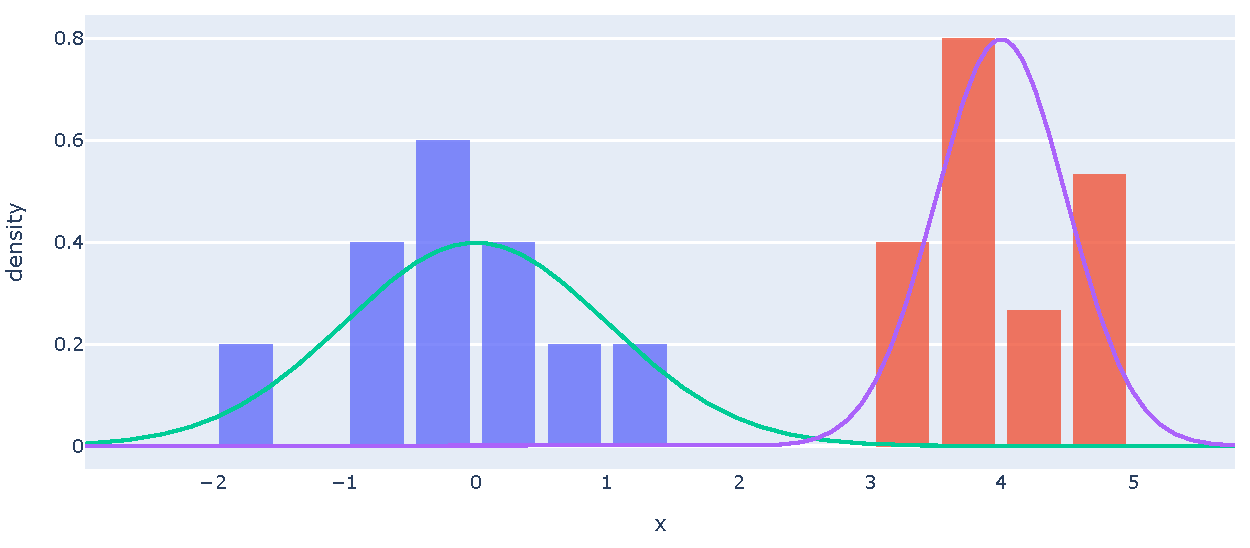
\includegraphics[width=0.8\textwidth]{imgs/p3.3.1.pdf}
	\caption{Muestras generadas para $X_1$ (azul) y $X_2$ (naranjo) junto a sus densidades originales.}
\end{figure}

Para las distribuciones continuas $X_1$ y $X_2$ se calculó el mapa de transporte óptimo desde $X_1$ a $X_2$ y su distancia de Wasserstein $W_2^2(X_1,X_2)$ utilizando las fórmulas entregadas en el enunciado.

Para las distribuciones discretas generadas por las muestras, se calculó la matriz de transporte óptimo $P$ entre ambas distribuciones. Es importante notar que la formulación discreta de Kantorovich no permite asociar a cada átomo de la distribución de origen un único átomo de la distribución de llegada (ya que cada átomo de $\alpha$ está relacionado con todos los átomos de $\beta$ según las filas de $P$). Por este motivo, para poder realizar una comparación del transporte óptimo discreto con el transporte óptimo continuo, se tomó el valor esperado en la transformación discreta: $\tilde{T}(x_i) = \mathbb{E}(T(x_i)) = \sum_{j=1}^m P_{ij}y_j$. Los resultados obtenidos se pueden ver en la Figura 7.

\begin{figure}[h]
	\centering
	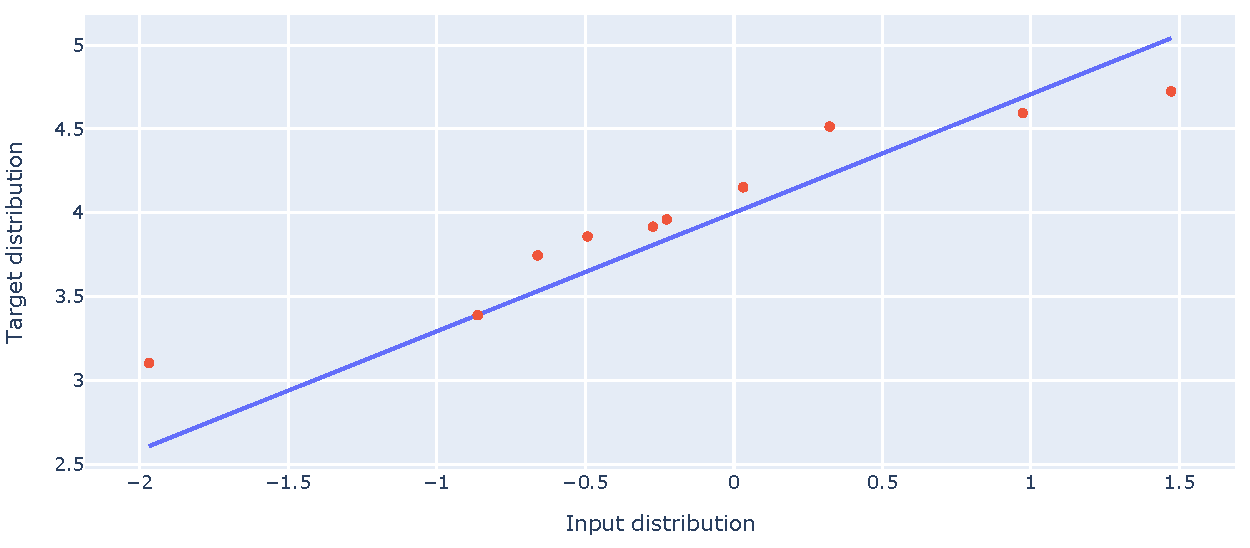
\includegraphics[width=0.8\textwidth]{imgs/p3.3.2.pdf}
	\caption{Transporte óptimo. En azul se ve el transporte óptimo teórico para las distribuciones continuas (mapa afín). En naranjo está el transporte óptimo (esperado) asociado a las distribuciones discretas.}
\end{figure}

\newpage
Por otra parte, los costos óptimos $W_2^2(X_1,X_2)$ obtenidos son los siguientes:

\begin{itemize}
	\item Costo mínimo teórico (distribución continua): $17.08$.
	\item Costo mínimo numérico (distribución discreta): $17.55$.
\end{itemize}

Se observa que ambos resultados estan muy cercanos, lo cual puede deberse a la baja varianza que se utilizó en el experimento, lo cual genera que pocas muestras sean representativas de la distribución.

\subsection{Análisis para el caso $d=2$}

En esta sección se estudiará el transporte óptimo para dos distribuciones discretas en $\mathbb{R}^2$. Estas corresponden a distribuciones empíricas formada por muestras generadas a partir de dos gaussianas independientes $X_1\sim\text{NMV}(\mu_1,\Sigma_1)$ y $X_2\sim\text{NMV}(\mu_2,\Sigma_2)$, donde:

\begin{equation*}
	\mu_1 = \begin{pmatrix} 0 \\ 0 \end{pmatrix}
	\quad
	\Sigma_1=\begin{pmatrix}
		1 & 0 \\
		0 & 1 \\
		\end{pmatrix}
	\qquad
	\mu_2 = \begin{pmatrix} 3 \\ 5 \end{pmatrix}
	\quad
	\Sigma_2=\begin{pmatrix}
		0.4 & 0.2 \\
		0.2 & 0.3 \\
		\end{pmatrix}
\end{equation*}
Las muestras generadas para ambas distribuciones pueden observarse en la Figura 8.

\begin{figure}[h]
	\centering
	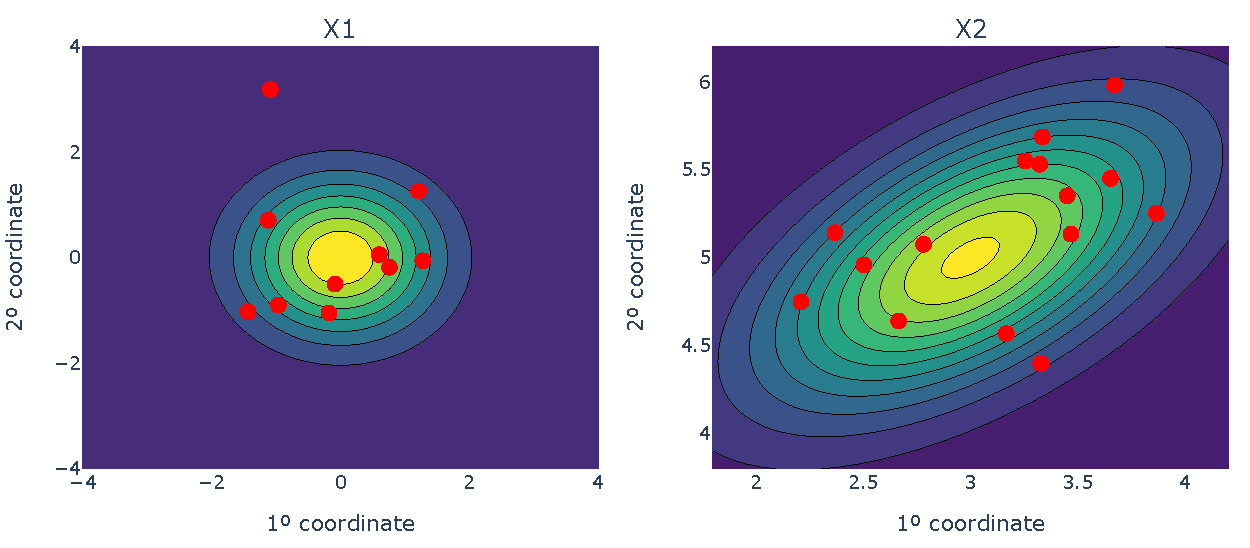
\includegraphics[width=0.9\textwidth]{imgs/p3.4.1.pdf}
	\caption{Mapa de calor de las densidades de $X_1$ y $X_2$. En rojo se observan las muestras generadas a partir de cada distribución.}
\end{figure}

\newpage
Dado que las distribuciones están definidas sobre $\mathbb{R}^2$, se visualizará el transporte óptimo de $\alpha$ a $\beta$ coordenada a coordenada. Los resultados obtenidos utilizando la formulación discreta de Kantorovich se pueden ver en la Figura 9.

\begin{figure}[h]
	\centering
	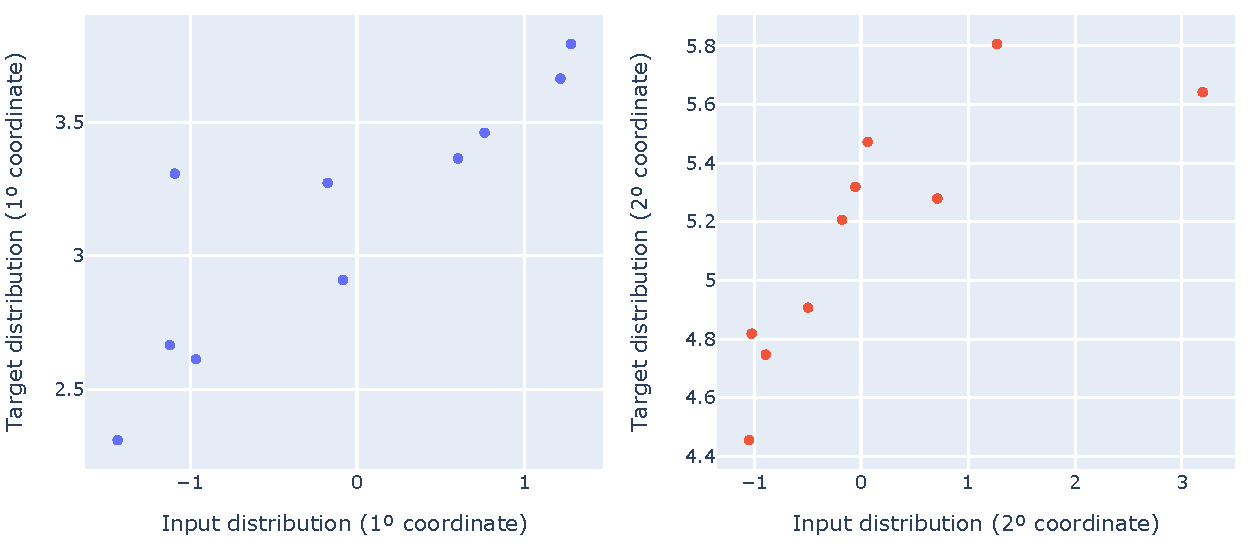
\includegraphics[width=0.8\textwidth]{imgs/p3.4.2.pdf}
	\caption{Transporte óptimo esperado desde la distribución discreta $\alpha$ a la distribución discreta $\beta$.}
\end{figure}

Se puede observar una tendencia lineal en cada componente del transporte óptimo. Esto es consistente con la solución óptima exacta, la cual indica que el transporte óptimo es un mapa afín entre ambas distibuciones.

\end{document}